%!TEX root = ./main.tex

\noindent Once the dataset generation has been completed, it can be used to train a neural network able to predict the final OCP cost. The data contained in the \texttt{.npz} file, although it has been prepared to be fed to the neural network, some preprocessing steps are required.

\noindent The first consists of removing the outliers present in the dataset. This was done by setting a threshold on the cost values and removing all samples with a cost higher than 20000. These samples were considered too far from the average cost value and would have negatively affected the training process.

\noindent The second step consisted in bounding both the inputs (denoted by $\mathbf{X}$) and the targets (denoted by $\mathbf{Y}$) to the range $[-1,1]$. This choice was motivated by the use of the \texttt{tanh} activation function in the neural network, whose output lies in the same interval. Moreover, neural networks generally perform better when the input data is normalized.

\noindent Additionally the targets, before scaling, were transformed using a logarithmic scale according to:
\begin{equation}
    \mathbf{Y}_{\text{log}} = \ln(\mathbf{Y} + 10^{-8})
\end{equation}

\noindent This transformation was introduced because the cost values spanned several orders of magnitude. Using a logarithmic scale helped to narrow the spread of the targets, making the training process more stable. The small constant $10^{-8}$ was added to avoid taking the logarithm of zero. Additionally, during preliminary tests, the network showed poor accuracy when predicting cost values close to zero. The logarithmic transformation significantly improved the prediction accuracy in this region.

\noindent When using the trained network to predict the final cost, the inverse transformation was applied in order to recover the actual cost values.

\noindent The dataset was then split into training and test sets, using 80\% of the samples for training and 20\% for testing. This split allowed us to monitor the performance of the network on unseen data during training and to reduce the risk of overfitting.
\\
\noindent The neural network architecture was defined as follows:
\begin{itemize}[noitemsep]
    \item One input layer with 4 neurons, corresponding to the state variables (position and velocity);
    \item Two hidden layers with 256 neurons each;
    \item One output layer with a single neuron representing the predicted cost;
    \item The \texttt{tanh} activation function was used for all layers.
\end{itemize}

\noindent The training process was implemented using batch gradient descent. For each training epoch, batches of $n = 256$ samples were drawn from the training set. For each batch, the network performed a forward pass, mapping the initial pendulum state to a predicted cost, followed by the computation of the Mean Squared Error (MSE), defined as:
\begin{equation}
    \text{MSE}(\mathbf{w}) = \frac{1}{n} \sum_{i=1}^{n} \left( \phi(\mathbf{x}_i, \mathbf{w}) - y_i \right)^2
\end{equation}
\noindent Where $\mathbf{w}$ denotes the network weights, $\phi(\mathbf{x}_i, \mathbf{w})$ is the predicted cost associated with the input state $\mathbf{x}_i$, and $y_i$ is the corresponding true cost value from the dataset.

\noindent For each batch within an epoch, the weights $\mathbf{w}$ were updated by applying the gradient descent to the MSE loss, this was implemented via the optimization algorithm Adam (Adaptive Moment Estimation) from the library PyTorch (\texttt{torch.optim.Adam}). It is important to distinguish this optimization algorithm from the ADAM robotics library used in Chapter \ref{cap1} for rigid body dynamics; while they share the same name, the former is an algorithm for training neural networks, whereas the latter is a software framework for kinematic and dynamic computations. The learning rate was initially set to $10^{-3}$ and progressively decayed down to a minimum value of $10^{-5}$ using a learning rate scheduler. In particular, PyTorch's \texttt{ReduceLROnPlateau} scheduler was employed, which reduces the learning rate when the test loss (defined in ~\eqref{eq:loss_test}) does not improve for a specified number of epochs. This strategy helped stabilize the training process and slightly improved the final performance.

\noindent At the end of each epoch, the training loss was computed as the average of the MSE values over all training batches:
\begin{equation}
    \text{Loss}_{\text{train}}(\mathbf{w}) = \frac{1}{m} \sum_{j=1}^{m} \text{MSE}_j(\mathbf{w})
\end{equation}
\noindent Where $m$ denotes the total number of batches in the training set. This metric was used to monitor the learning progress.

\noindent The testing procedure followed the same structure as the training process, with the only difference being that the network weights were not updated. The test loss was computed as
\begin{equation}
    \label{eq:loss_test}
    \text{Loss}_{\text{test}}(\mathbf{w}) = \frac{1}{m} \sum_{j=1}^{m} \text{MSE}_j(\mathbf{w})
\end{equation}
\noindent Where $m$ is the number of batches in the test set.

\noindent The entire training process was repeated for a total of 600 epochs. Both training and testing losses were monitored throughout the training, and the resulting trends are shown in Figure~\ref{fig:loss}.

\FloatBarrier
\begin{figure}[htbp]
    \centering
    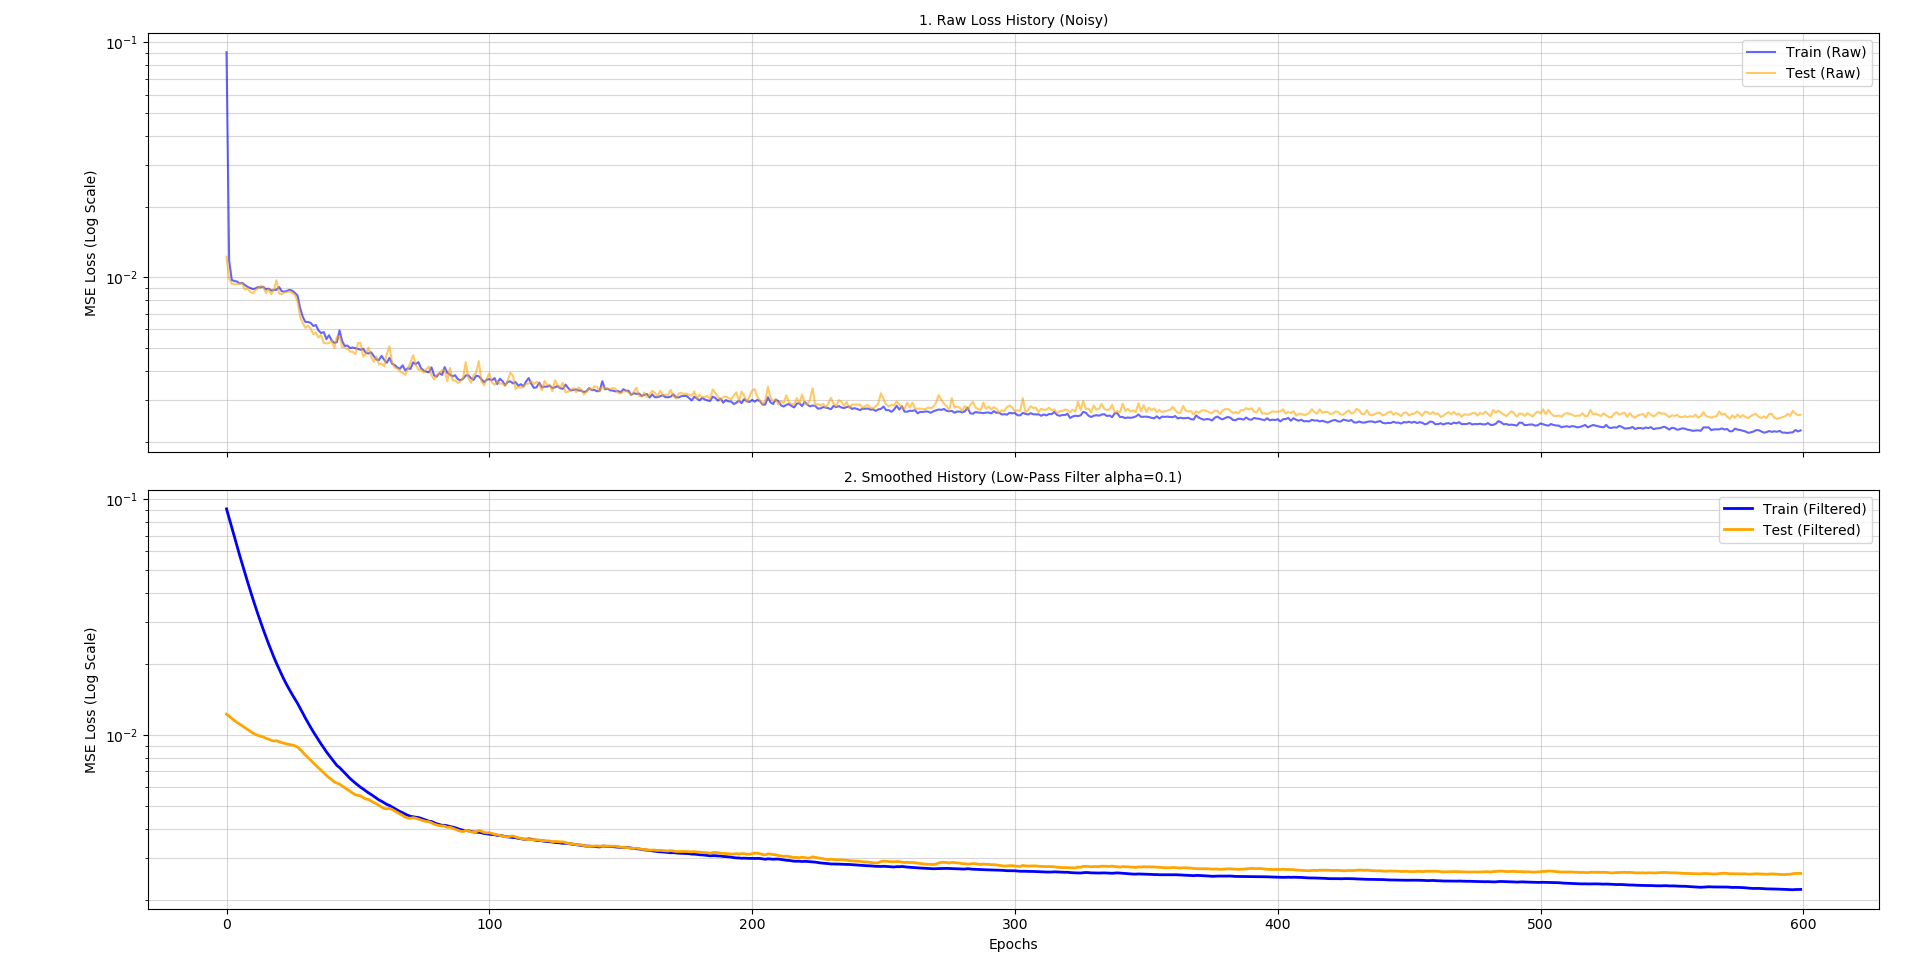
\includegraphics[width=0.9\textwidth]{pics/loss_plot.png}
    \caption{Training and testing losses over the training epochs.}
    \label{fig:loss}
\end{figure}

\noindent As shown in the figure, a low-pass filter was applied to the loss curves to better visualize their overall trends. The training loss decreases steadily over the epochs, indicating that the network effectively learns from the training data. The testing loss follows a similar decreasing trend, suggesting good generalization performance and the absence of significant overfitting.

\noindent An example of the code used during the training process is reported in Figure~\ref{fig:code_example_train}.


\begin{figure}[H]
    \centering
    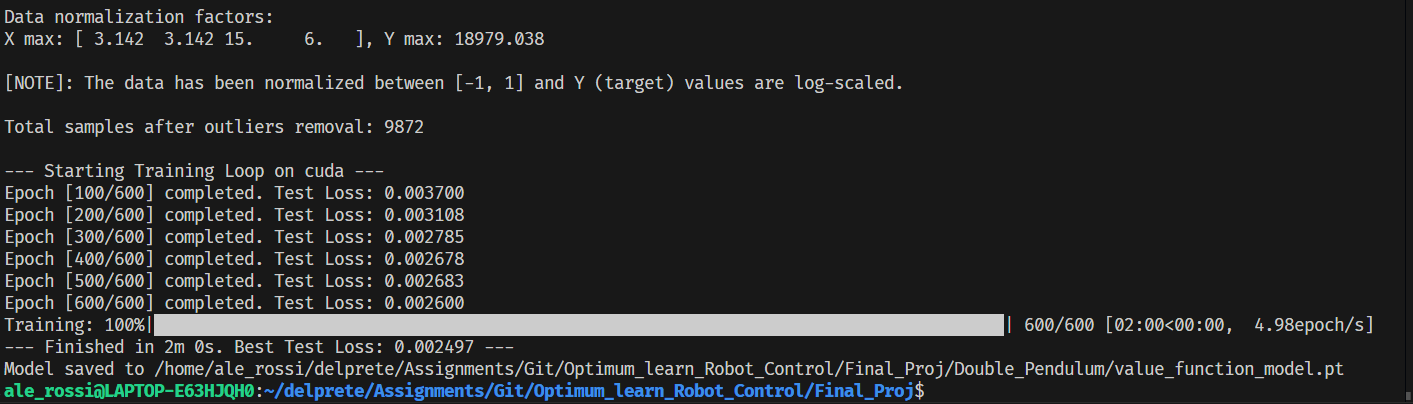
\includegraphics[width=0.9\textwidth]{pics/train_bono.png}
    \caption{Example of code used for the training process.}
    \label{fig:code_example_train}
\end{figure}

\noindent The overall training procedure required approximately two minutes to complete, thanks to the use of GPU acceleration available on one of the laptops.
\\

\noindent All of this was implemented in the file: "\texttt{fase2\_network\_training\_doub\_pend.py}"
